\documentclass[a4paper]{article} 
\usepackage{geometry,fancyhdr,subfig,listings,graphicx,psfrag,amsfonts,textcomp,mathtools,amsmath,hyperref} 

\title{Mandatory exercise 4 \\
Signal and Image Processing 2012} 
\author{Jens P. Raaby \\
\url{frn617@diku.dk}}

\begin{document} 
\maketitle

\section*{Question 4.1 - Gamma Correction} To implement the user interface I used the GUIDE tool in Matlab. The image (in the form of an M x N array of pixels) is passed to the tool via an argument, for example 
\begin{lstlisting}
	gammatool(imread('barbara.tif')); 
\end{lstlisting}

The result of loading the tool is shown in the figure \ref{q1demo}, and the source code is listed in appendix \ref{appendix-gammatool}. I set the slider component to take input in the range -1 to 1, which are applied as exponents of 10 to give gamma values in the range 0.1 to 10.
\begin{figure}
	\centering 
	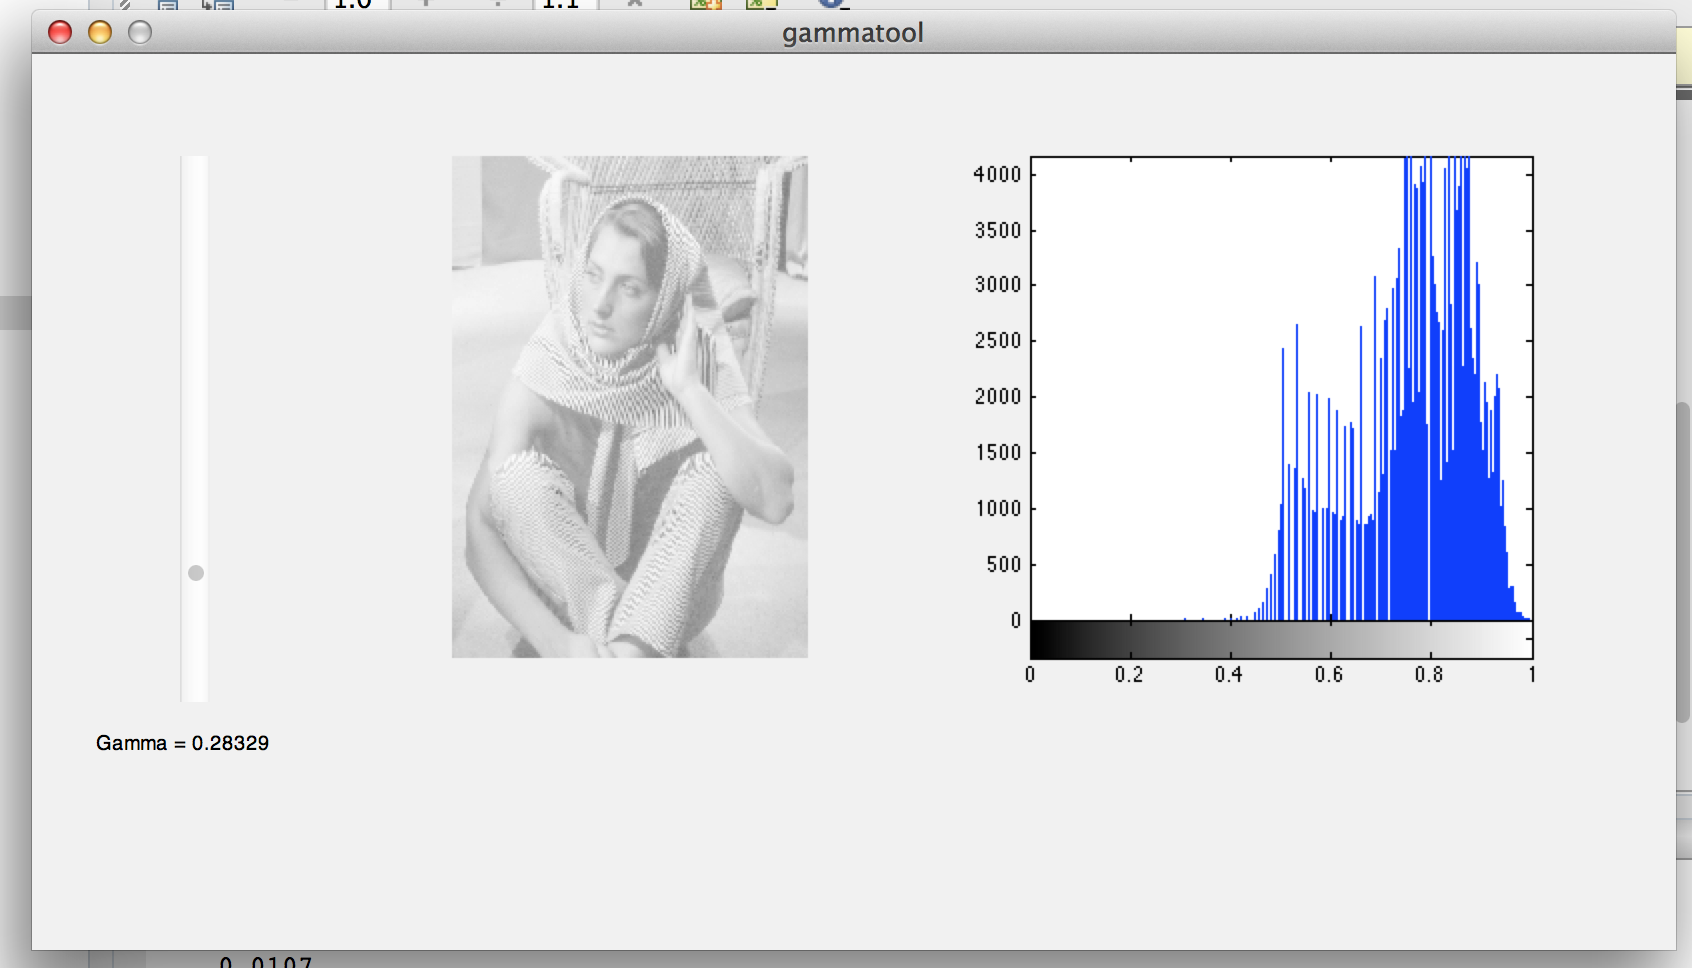
\includegraphics[width=0.7
	\textwidth]{gammatool.png} \caption{Demonstration of the Gamma tool developed for Q4.1} \label{q1demo} 
\end{figure}
\section*{Question 4.2 - Monotonic intensity changes} Deriving the equations for a strictly decreasing intensity. 
This means the cumulative probability distribution still sums to 1, but has the opposite gradient and thus the probability density function is inverted. The function $g$ is strictly decreasing and has an inverse, then that function is also decreasing.
The domain and range of the inverse function can thus be expressed:
\begin{equation}
	g^{-1}(( -\infty, s]) = [g^{-1}(s),\infty)    
\end{equation}
Since $s = g(r)$ and $r = g^{-1}(s)$, 
\begin{equation}
    P_S(s) = P(R \in [g^{-1}(s), \infty))
    \label{PrRange}
\end{equation}

\begin{equation}
    P_S(g(r)) = P_R(r) \Leftrightarrow P_S(s) = P_R(g^{-1}(s))
    \label{PsPr}
\end{equation}

We have the definition of $P_R(t)$ (it always takes value 1), and since we know the integration intervals in this decreasing case from above:
\begin{equation}
    P_R(t) = \int_t^\infty p_r(x) dx + \int_{-\infty}^t p_r(x) dx = 1
    \label{sumint}
\end{equation}
\begin{equation}
    P_R(t) = \int_{-\infty}^\infty p_r(x) dx = 1
\end{equation}
Hence from (\ref{PsPr}) and (\ref{sumint}):
\begin{equation}
    P_S(t) = 1 - P_R(t) = 1 - P_R(g^{-1}(s))
\end{equation}
This follows because $P_R$ can be expressed as the sum of the two integrals, and it always takes value 1. Since we know $P_R$ is the integral of a decreasing function, and we know its range from (\ref{PrRange}), then this is rearranged as $1 - P_R(t)$.

Now the derivatives can be calculated:

\begin{equation}
\frac{d(P_S(t))}{dr} = \frac{d(P_S(g(r)))}{dr} = \frac{d(1-P_R(r))}{dr} 
\end{equation}
Beginning with the right hand side:
\begin{equation}
     \frac{d(1-P_R(r))}{dr} = -p_R(r)
\end{equation}
The left side can be derived using the chain rule:
\begin{equation}
    \frac{d(P_S(g(r)))}{dr} = p_S(s) \frac{d(g(r))}{dr} = p_S(s)\frac{ds}{dr}
\end{equation}
%%%%%%%%%%%%%%%%%%%%%
\section*{Question 4.3 - More maths} Compare results to those when intensity transforming and image with function g.

\section*{Question 4.4 - Hisogram equalisation and matching} Discuss potential problems due to quantization/rounding and solutions to them.

\section*{Question 4.5 - RGB to HSI and Back again} Is there a simpler way than using conversion to and from HSI?

\appendix 
\section{Gammatool source} \label{appendix-gammatool} \lstinputlisting{gammatool.m} \end{document} 
